% !TEX root=../index.tex


\chapter{Gestore dei Dataset} % (fold)
\label{chap:training_set_creator}
    Si tratta di un'applicazione desktop che consente di gestire efficacemente i vari dataset.
    Una volta aperto, nella schemata principale (figura \ref{fig:tsc_main}) gli elementi vengono organizzati in una tabella che ne riporta l'id numerico, le dimensioni e l'etichettatura reale.
    \begin{figure}[h]
        \centering
        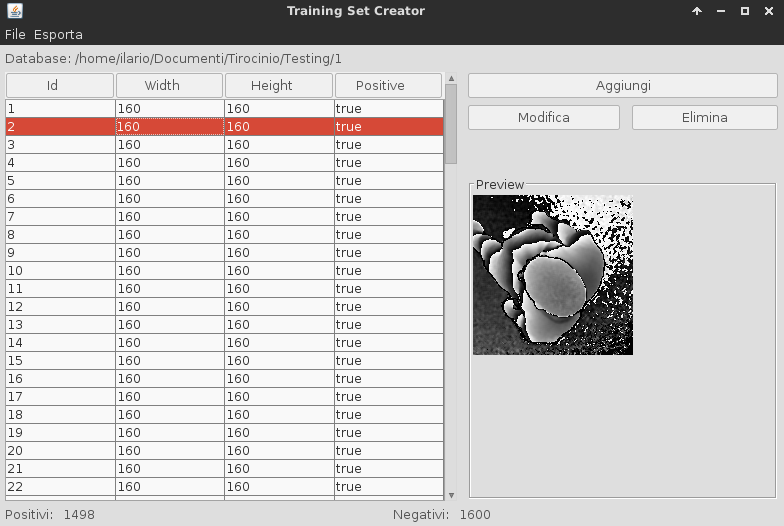
\includegraphics[width=10cm]{img/training_set_creator_main.png}
        \caption{Schermata principale del software di gestione.}
        \label{fig:tsc_main}
    \end{figure}

    Di ogni elemento, una volta selezionato, è disponibile una piccola preview.
    Inoltre sono disponibili le elementari azioni di modifica (che consiste nel cambiare l'etichettatura dell'elemento in caso di errore) e cancellazione per ognuno di essi.

    Premendo il bottone \emph{Aggiungi} si attiverà la procedura per l'aggiunta degli elementi al dataset. 
    Si aprirà una schermata in cui verrà richiesto di selezionare la cartella contenente le registrazioni effettuate con il Kinect.
    Poichè ogni frame viene salvato in un file binario privo di qualsiasi metadato, non è possibile risalire alla risoluzione originale del frame e sarà necessario specificarla manualmente. 

    Inseriti i dati necessari si aprirà l'interfaccia in figura \ref{fig:tsc_add} che permetterà di scorrere tra i frame della registrazione utilizzando la scrollbar in alto e selezionare la porzione di frame desiderata evidenziandola con il mouse, così come si farebbe in un qualsiasi programma di photo editing.
    \begin{figure}[h]
        \centering
        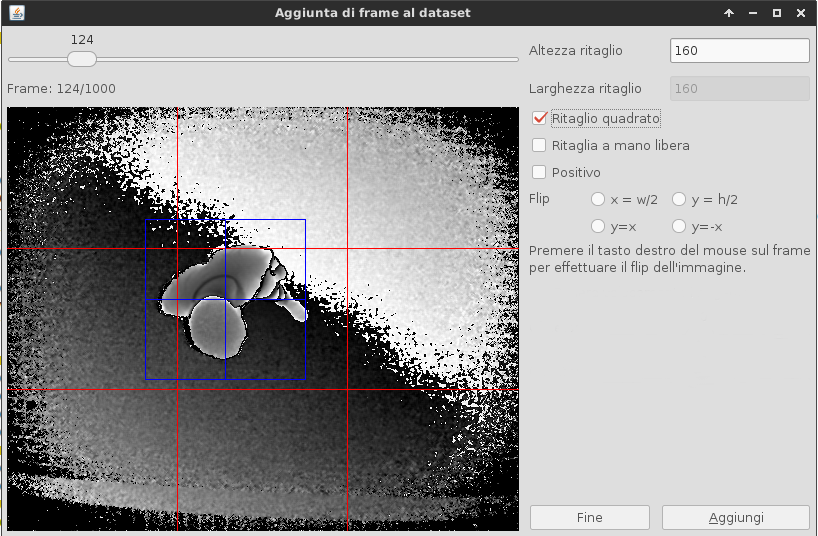
\includegraphics[width=10cm]{img/training_set_creator_add.png}
        \caption{Schermata per l'aggiunta di un nuovo elemento al dataset.}
        \label{fig:tsc_add}
    \end{figure}

    È disponibile anche la funzionalità per il resize delle immagini, raggiungibile dalla voce \emph{Resize} del menu \emph{Esporta}.

    \begin{figure}[h]
        \centering
        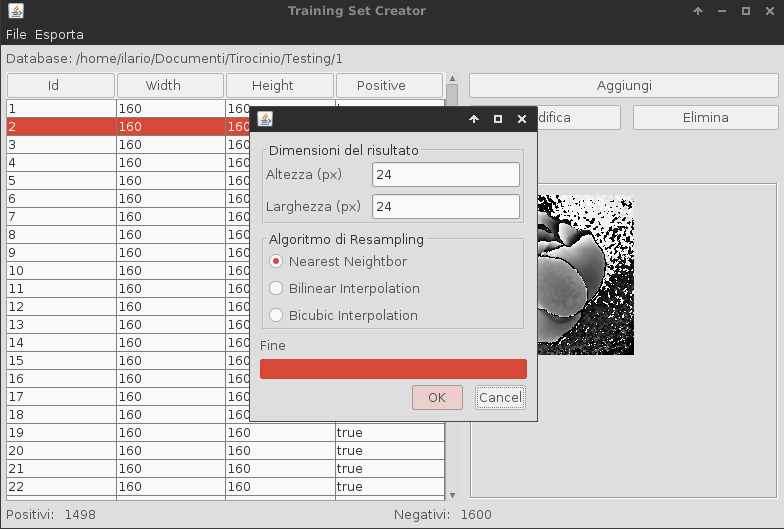
\includegraphics[width=10cm]{img/training_set_creator_resize.png}
        \caption{Schermata per il resize degli elementi del dataset.}
        \label{fig:tsc_resize}
    \end{figure}

    Nella schermata in figura \ref{fig:tsc_resize} sarà necessario inserire le nuove dimensioni per le immagini e selezionare l'algoritmo di resampling desiderato.

    Il software è stato scritto in linguaggio Java, utilizzando il pattern \emph{Model View Controller}.
    Questo approccio mira a dividere il codice in blocchi funzionali ben distinti, ognuno con un obiettivo ben specifico:
    \begin{description}
        \item[Model] Le classi che lo compongono implementano la \emph{business logic} dell'applicazione, ovvero si occupano della modellazione degli oggetti della realtà di interesse in oggetti software e descrivono le operazioni eseguibili su di essi.

        \item[View] Tutte le interfacce grafiche vengono raggruppate in questo modulo software. Vengono implementati i metodi per il popolamento delle viste e l'estrazione dei valori inseriti nei campi di input dall'utente.

        \item[Controller] Le classi di controllo si frappongono tra quelle del \emph{model} e quelle della \emph{view}, governando i meccanismi di rappresentazione dei dati all'utente e la loro modifica a fronte di un'azione intrapresa da quest'ultimo.
    \end{description}

    Questo approccio alla scrittura del software permette la realizzazione di un prodotto modulare, facilmente manutenibile ed espandibile.

    Per la persistenza dei dati e soprattutto dei metadati relativi agli elementi dei dataset, si è scelto di non utilizzare alcun meccanismo di persistenza centralizzato (\emph{DBMS} o file \emph{XML}), ma di rappresentare i metadati codificandoli nei nomi dei file.

    Ogni dataset, infatti, risiede in una specifica cartella.
    Al suo interno saranno presenti le sotto cartelle \emph{positives} e \emph{negatives}, che organizzeranno il file con i ritagli delle immagini di profondità in base alla loro reale classificazione.
    Il nome di ogni ritaglio è composto da una serie di parametri separati dal carattere \emph{underscore} e serializza lo stato del relativo oggetto software che lo modella all'interno dell'applicazione (\ref{eq:samples_filename}).

    \begin{equation}
        \label{eq:samples_filename}
        nome_{sample} = sample\_<id>\_<width>\_<height>\_<label>.bin
    \end{equation}
    
\chapter{Annotazioni sulla Suite di Training e Testing}
    \section{Utilizzo} % (fold)
    \label{sec:utilizzo}
        Il codice della suite software risiede nella cartella \emph{matlab} e nelle relative sotto cartelle.
        Per installarla\footnote{Per informazioni più specifiche riguardo alla compilazione delle librerie ed all'installazione della suite, si rimanda alla lettura del file \emph{README.md} contenuto nella root del progetto.} è sufficiente aggiungere ricorsivamente il percorso della prima alla variabile \emph{PATH} dell'ambiente Matlab.

        All'interno della cartella \emph{matlab/procedures} vi è la definizione degli script.
        Questi ultimi costituiscono a tutti gli effetti l'interfaccia che l'utente avrà a disposizione per l'utilizzo del sistema.
        Tali script richiamano una serie di funzioni, che vengono definite, per mantenere il codice leggibile e manutenibile, nelle altre sotto cartelle, divise per ambito d'utilizzo.

        Di seguito viene presentata la sequenza con il quale gli script vengono richiamati, in modo da percorrere l'intero workflow del sistema.
        \begin{description}
            \item[trainWithAdaboost] Esegue l'allenamento dell'algoritmo utilizzando il dataset di training predefinito\footnote{Consultare \emph{README.md}, specialmente la sezione relativa alla configurazione del file \emph{initEnvironment.m}.}.
            I classificatori forti estratti vengono serializzati e salvati in una cartella dal nome $strong\_classifier\_<datetime>$\footnote{Tutte le procedure successive, sono in grado di deserializzare lo strong learner, data tale path.}, all'interno dell'attuale directory di lavoro.

            \item[evaluateClassifierThresholds] Valuta le prestazioni dei classificatori facendo variare la soglia e il numero di weak learner.
            Salva automaticamente i risultati all'interno della path dei classificatori.

            \item[strongClassifierTuning] Utilizzando i dati ottenuti al passo precedente, sceglie i parametri ottimali per la regolazione.

            \item[testAdaboost] Una volta che il sistema è stato allenato ed è stato effettuato il tuning, è possibile lanciare questo script per testarne le prestazioni complessive.

            \item[detectHumanInFrames] Script per il rilevamento della persona all'interno dei frame delle registrazioni.
            È possibile effettuare rilevamenti sia su frame singoli o che su frame sequenzialmente correlati.
        \end{description}
    % section utilizzo (end)


    \section{Implementazione dell'Algoritmo di Allenamento}
        Il linguaggio Matlab permette di sviluppare software molto velocemente grazie alla miriade di funzionalità messe a disposizione dalle librerie standard, che consentono di tralasciare molti dettagli implementativi e concentrare gli sforzi sullo sviluppo della logica di business.
        Tuttavia la fase di allenamento è la più pesante dal punto di vista computazionale, sia per la complessità intrinseca dell'algoritmo, che per la mole di dati in ingresso, quindi richiede un approccio differente.

        In Matlab alcune funzioni possono essere implementate in un altro linguaggio ad alto livello (come il C++, il Java o il FORTRAN) attraverso l'uso dei \emph{file mex}, al fine di migliorne le prestazioni.
        Una volta scritto il file sorgente della funzione nel linguaggio scelto, lo si compila utilizzando il compilatore in dotazione con la suite Matlab, generando così il file mex che verrà linkato dinamicamente in fase di esecuzione.

        È stata quindi sviluppata una libreria di supporto in C++ che implementa le parti più critiche dell'algoritmo di allenamento.
        Tale liberia viene poi utilizzata nelle funzioni implementate nei file mex e queste ultime verranno richiamate negli script in Matlab.

        \lstinputlisting[language=c++, frame=single]{code/best_weak_classifier.cxx}

        In questa piccola porzione di codice, relativa alla funzione compilata per la selezione del miglior weak learner, mostra l'utilizzo del metodo \emph{bestWeakClassifier} della classe \emph{Adaboost} definita in \emph{adaboost.h}.